\documentclass[14pt, a4paper]{extarticle}
\usepackage[14pt]{extsizes}
\usepackage[utf8]{inputenc}
\usepackage[russian]{babel}
\usepackage{amsmath}
\usepackage{amsfonts}
\usepackage{graphicx}
\usepackage{amssymb}
\usepackage[left=2cm,right=2cm,top=2cm,bottom=2cm,bindingoffset=0cm]{geometry}
\usepackage{graphicx}
\usepackage[T2A]{fontenc} 
\usepackage{multicol}
\usepackage{caption}
%\usepackage{subcaption}
\usepackage{textcomp} 
\usepackage{setspace} 
\usepackage{chngcntr}
\usepackage[small]{titlesec} 
\setlength{\parindent}{1.25cm}
\renewcommand{\baselinestretch}{1.3}
\usepackage{cmap}
\AtBeginDocument{\let\textlabel\label}
\usepackage{hyperref}
\hypersetup{pdftex,colorlinks=true,linkcolor = black, citecolor = blue, backref=page}
\usepackage[all]{hypcap}

\usepackage{subfig}
\graphicspath{ {img/} }

%\bibliographystyle{gost780u}
\bibliographystyle{unsrt}

%\counterwithin{equation}{section}
\renewcommand{\theequation}{\arabic{section}.\arabic{subsection}.\arabic{equation}}
\newcommand{\RNumb}[1]{\uppercase\expandafter{\romannumeral #1\relax}}
\begin{document}
	\begin{titlepage}
		\begin{center}
			\hfill \break
			МОСКОВСКИЙ ФИЗИКО-ТЕХНИЧЕСКИЙ ИНСТИТУТ\\ (ГОСУДАРСТВЕННЫЙ УНИВЕРСИТЕТ)\\
			\hfill \break
			\hfill \break
			\hfill \break
			\hfill \break
			\hfill \break
			Департамент философии\\
			\hfill \break
			\hfill \break
			РЕФЕРАТ ПО ИСТОРИИ НАУКИ\\
			\hfill \break
			\hfill \break
			\large{\textbf{История развития и проблемы биометрического распознавания человека}}\\
			\hfill \break		
		\end{center}
		
		\begin{center}
			\hfill \break
			\parbox{0.9\textwidth}
			{
				Аспирант~--- Соломатин Иван Андреевич \\
				Научный руководитель аспиранта \underline{\hspace{3cm}} д.т.н. Матвеев И.А. \\
				Преподаватель департамента философии~--- Фурсов А.А. \\
			}
		\end{center}
		\hfill \break
		\hfill \break
		\hfill \break
		\hfill \break
		\begin{center} Москва, 2018 
		\end{center}
		\thispagestyle{empty} 
	\end{titlepage}
	
\tableofcontents
\newpage

\section{Введение}
На протяжении всей истории человечества задача распознавания человека была актуальной, однако в последние годы интерес к ней многократно возрос. В основном, это вызвано появлением новых технических средств и всё более глубоким их проникновением в повседневную жизнь людей. Набор технических приёмов, применяемых для распознавания человека по физическим и поведенческим параметрам в наше время принято называть \textit{биометрией}. Появившиеся технические возможности открывают новые методики и совершенно новые и неожиданные сферы применения биометрии. В современном виде биометрия стала применяться с конца \texttt{XIX} века в криминалистике. В настоящее время слово "биометрия"\ у всех на слуху: биометрическое распознавание используется в смартфонах \cite{odinokikh2018high, sezan2014user, hwang2009keystroke}, в банковском деле \cite{fatima2011banking, venkatraman2008biometrics}, в маркетинге \cite{?},
%в криминалистике \cite{tistarelli2014biometrics, bouchrika2011using},
в социологии (в сфере социального управления) \cite{?}.

Сама постановка задачи распознавания человека по каким-либо признакам имеет глубокие корни, уходящие далеко в прошлое. На самом деле, любой человек, не задумываясь, решает эту задачу каждый день по многу раз, когда узнаёт своих родных, друзей, коллег. Чаще всего, при социальном взаимодействии, человек выстраивает диалог и предпринимает те или иные действия исходя из знания того, с кем именно он взаимодействует. Таким образом, данная задача лежит в основе социального взаимодействия людей и именно поэтому она настолько актуальна и обсуждаема.

В данной работе описывается история развития различных систем распознавания, а так же некоторые проблемы, связанные с подобными системами.

\newpage
\section{Постановка задачи распознавания человека}

\newpage
\section{История развития систем распознавания человека}
Как было сказано выше, задача распознавания человека была актуальной испокон веков. До появления науки биометрии людям тоже нужно было идентифицировать себя и подтверждать свою личность (аутентифицировать) и для этого изобретались различные устройства и системы.
Например, для подтверждения авторства писем ещё в конце \texttt{IV} века в Риме начали использовать сургучные печати. Печати используются для подтверждения подлинности документов и по сей день.

Больший же интерес для данной работы представляют системы именно биометрического распознавания, то есть распознавания по физическим и поведенческим параметрам. Существует множество параметров, по которым можно построить систему биометрического распознавания человека, такие параметры называются биометрическими модальностями. И, как следствие, существует множество разновидностей таких систем. Ниже описывается история развития систем распознавания по основным биометрическим модальностям, которые активно используются в наше время, или активно использовались в прошлом.

\subsection{Бертильонаж}
Бертильонаж~--- система идентификации человека по антропометрическим данным. Названа в честь своего изобретателя~--- Альфонса Бертиль\'{о}на.

Работая писарем в полиции Парижа и переписывая карточки с описанием преступников, Альфонс Бертильон обратил внимание на то, что данные описания являются крайне поверхностными и нечёткими, например "высокого роста", "плотного телосложения", и т.п. Бертильон предложил использовать для идентификации преступников точные измерения различных частей тела. Проведя серию экспериментов, он предложил использовать для этого метода следующие параметры: длина головы, ширина головы, длина среднего пальца, длина левой ступни и длина локтя \cite{bertillon}. Впервые система была успешно использована создателем 20 февраля 1883 года, когда он опознал в одном из заключённых преступника, который уже был осуждён ранее и измерен. Но по настоящему большую известность система получила 30 марта 1892, когда с её помощью удалось обнаружить и арестовать организатора серии террористических актов в Париже.
Система с успехом применялась Французской полицией до 1914 года~--- года смерти Бертильона. После его смерти, место бертильонажа заняла дактилоскопия, или распознавание по отпечаткам пальцев.
\subsection{Распознавание по отпечаткам пальцев}
Распознавание по отпечаткам пальцев~--- первая научно обоснованная методика биометрического распознавания. Она основана на уникальности рисунка на пальцах человека, называемого папиллярным узором. На рис. \ref{img:fingerprints} изображены примеры этих узоров.

\begin{center}
	\begin{figure}[h!]
		\centering
		\subfloat[Петля]{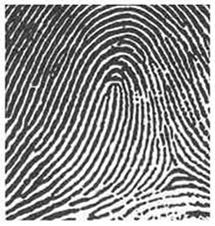
\includegraphics[width=0.25\textwidth]{fingerprint_1.png}}
		\hspace{0.05\textwidth}
		\subfloat[Дуга]{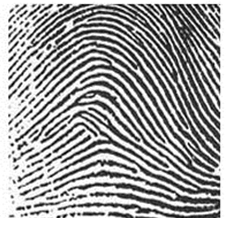
\includegraphics[width=0.25\textwidth]{fingerprint_2.png}}
		\hspace{0.05\textwidth}
		\subfloat[Завиток]{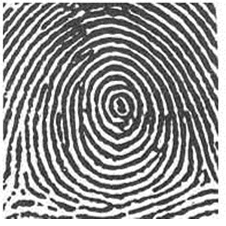
\includegraphics[width=0.25\textwidth]{fingerprint_3.png}}
		\caption{Примеры папиллярных узоров различных типов}
		\label{img:fingerprints}
	\end{figure}
\end{center}

\vspace{-1cm}

Первое упоминание об использовании отпечатков пальцев относится к древним временам. Уже в древнем Вавилоне и древнем Китае люди использовали эти уникальные узоры для подписи документов. Кроме того, согласно работе \cite{xiang1988historical}, историки нашли свидетельство того, что в Китае уже в конце \texttt{III} века до нашей эры, отпечатки пальцев использовались в криминалистике для идентификации преступников. 

Впервые папиллярные узоры на пальцах человека были описаны итальянским биологом и врачом Марчелло Мальпиги в его работе \cite{malpighi1669opera}, датированной 1669 годом. Первое упоминание о том, что рисунок папиллярных линий пальца является уникальным для каждого человека принадлежит Иоганну Кристофу Андреасу Майеру, который написал об этом в своей работе по анатомии \cite{mayer1794anatomische}, опубликованной в 1794 году. 

В 1823 году чешский учёный Ян Эвангелиста Пуркинье опубликовал работу \cite{purkynve2013dissertation}, в которой впервые предлагалась классификация папиллярных узоров, содержащая девять основных типов узоров, которая заложила фундамент современной дактилоскопии. 

Одним из основоположников дактилоскопии является Уильям Хершел, который доказал, что узор на пальцах не меняется на протяжении жизни человека, а так же после его смерти. С 1858 года Хершел, работавший чиновником в Индии, начал использовать отпечатки пальцев для подтверждения подлинности документов. В 1877 г. он предложил использовать отпечатки пальцев для регистрации заключённых. Это был первый случай научно обоснованного практического использования дактилоскопии.

В наше время существует множество алгоритмов, позволяющих распознавать человека по отпечатку пальца в автоматическом режиме. Такие алгоритмы используются как в криминалистике, так и в повседневной жизни людей: в большинстве смартфонов, в персональных компьютерах, биометрических замках, и т.д.

\subsection{Распознавание по радужной оболочке глаза}
Радужка~--- передний отдел сосудистой оболочки глазного яблока, видимый через прозрачную роговицу \cite{petrovskiy1974bme}. Радужка имеет яркую окраску и обладает слабо меняющуейся со временем структурой, которая содержит в себе одни из наиболее надёжных признаков для распознавания человека. Регистрацию изображения радужной оболочки можно произвести дистанционно и неинвазивно с использованием не слепящей направленной подсветки. Данная биометрическая модальность считается самой эффективной на данном этапе развития биометрии \cite{gupta2011iris}.

Первое упоминание об использовании радужной оболочки для распознавания личности принадлежит глазному хирургу Франкe Буршe, и было сделано в 1936 году \cite{misztal2012iris}


\begin{center}
\begin{figure}[h!]
	\centering
	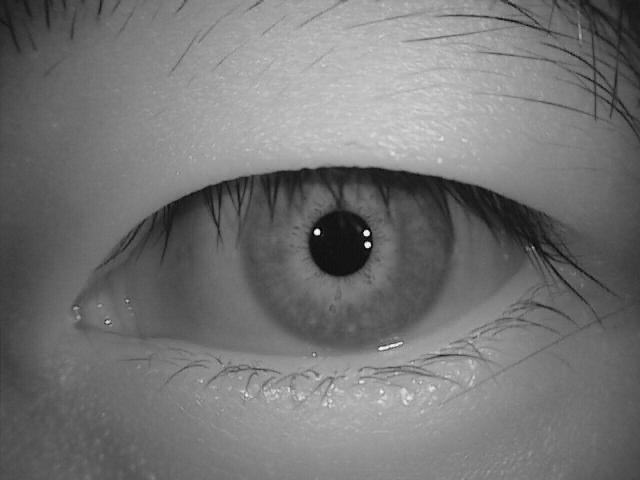
\includegraphics[width=0.45\textwidth]{iris_sample_1.png}
	\hspace{0.05\textwidth}
	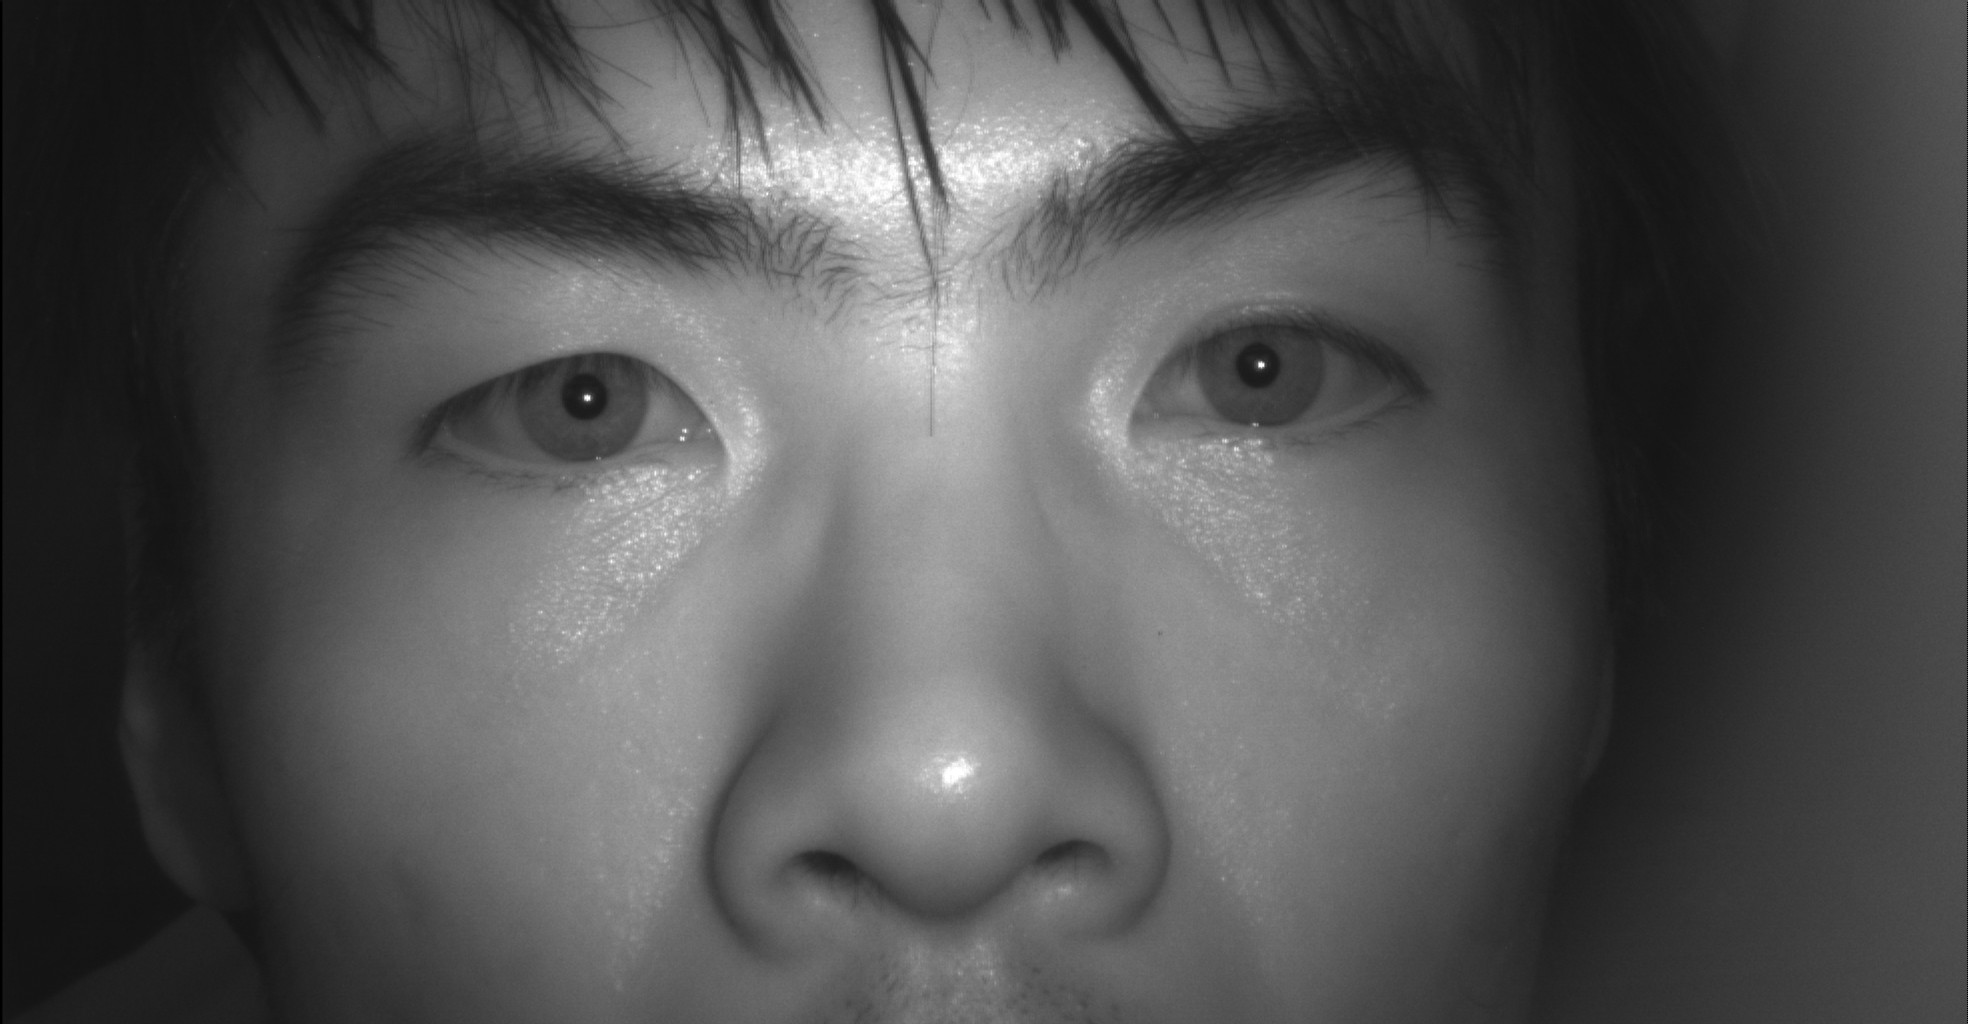
\includegraphics[width=0.45\textwidth]{iris_sample_2.png}
	\caption{Примеры изображений, используемых для распознавания человека по радужной оболочке.}
	\label{img:iris_samples}
\end{figure}
\end{center}
\vspace{-1cm}`
На основе его исследований офтальмологи Л. Флом и А. Сафир в 1987 г. запатентовали основные принципы распознавания по радужной оболочке \cite{flom1987iris}. Для разработки алгоритма А. Сафир и Л. Флом обратились за помощью к Джону Даугману, который, впоследствии, в 1994 г. запатентовал первую систему идентификации личности по изображению радужки \cite{daugman1994biometric}, и считается родоначальником этого вида распознавания. Основными этапами работы алгоритма, запатентованного Даугманом являются распознавания являются сегментация радужки, выделение признаков в этой области, их кодирование и классификация.
Большинство систем распознавания по радужной оболочке используют изображения, полученные в ближнем инфракрасном диапазоне, поскольку радужная оболочка в этом случае содержит меньшее количество бликов и имеет более контрастную структуру \cite{Daugman02}. Примеры изображений радужной оболочки приведены на рис. \ref{img:iris_samples}.

В последнее время алгоритм Даугмана начинает постепенно уступать в скорости и точности распознавания новым алгоритмам, которые используют искуственные нейронные сети.

В настоящее время распознавание по радужной оболочке используется в мобильных устройствах \cite{odinokikh2018high}, в биометрических замках, и в различных системах контроля доступа.

\subsection{Распознавание по лицу}
Распознавание человека по лицу~--- самый естественный метод биометрического распознавания, поскольку именно так мы привыкли узнавать друг друга в повседневной жизни. История изучения этой биометрической модальности, в отличие, например, от отпечатков пальцев, началась только с появлением ЭВМ. До появления ЭВМ узнать человека по фотографии или рисунку не составляло особого труда, поскольку любой человек умеет это делать от природы, и ему не требуются для этого какие-то алгоримы, но, с появлением ЭВМ возник вопрос: как научить компьютер распознавать лица? Именно в направлении ответа на этот вопрос и велись исследования в области данной биометрической модальности.


\subsection{Распознавание по голосу}
\subsection{Распознавание по походке}
\subsection{Распознавание по клавиатурному почерку (Стилометрия)}
\subsection{Тест ДНК}
\subsection{Распознавание по форме ушной раковины}
\subsection{Мультимодальные биометрические системы}

\newpage
\section{Проблемы биометрического распознавания человека}

\newpage
\section{Заключение}
	
\newpage
\bibliography{bibliography}

\end{document}
